\documentclass[twoside]{book}

% Packages required by doxygen
\usepackage{fixltx2e}
\usepackage{calc}
\usepackage{doxygen}
\usepackage[export]{adjustbox} % also loads graphicx
\usepackage{graphicx}
\usepackage[utf8]{inputenc}
\usepackage{makeidx}
\usepackage{multicol}
\usepackage{multirow}
\PassOptionsToPackage{warn}{textcomp}
\usepackage{textcomp}
\usepackage[nointegrals]{wasysym}
\usepackage[table]{xcolor}

% Font selection
\usepackage[T1]{fontenc}
\usepackage[scaled=.90]{helvet}
\usepackage{courier}
\usepackage{amssymb}
\usepackage{sectsty}
\renewcommand{\familydefault}{\sfdefault}
\allsectionsfont{%
  \fontseries{bc}\selectfont%
  \color{darkgray}%
}
\renewcommand{\DoxyLabelFont}{%
  \fontseries{bc}\selectfont%
  \color{darkgray}%
}
\newcommand{\+}{\discretionary{\mbox{\scriptsize$\hookleftarrow$}}{}{}}

% Page & text layout
\usepackage{geometry}
\geometry{%
  a4paper,%
  top=2.5cm,%
  bottom=2.5cm,%
  left=2.5cm,%
  right=2.5cm%
}
\tolerance=750
\hfuzz=15pt
\hbadness=750
\setlength{\emergencystretch}{15pt}
\setlength{\parindent}{0cm}
\setlength{\parskip}{3ex plus 2ex minus 2ex}
\makeatletter
\renewcommand{\paragraph}{%
  \@startsection{paragraph}{4}{0ex}{-1.0ex}{1.0ex}{%
    \normalfont\normalsize\bfseries\SS@parafont%
  }%
}
\renewcommand{\subparagraph}{%
  \@startsection{subparagraph}{5}{0ex}{-1.0ex}{1.0ex}{%
    \normalfont\normalsize\bfseries\SS@subparafont%
  }%
}
\makeatother

% Headers & footers
\usepackage{fancyhdr}
\pagestyle{fancyplain}
\fancyhead[LE]{\fancyplain{}{\bfseries\thepage}}
\fancyhead[CE]{\fancyplain{}{}}
\fancyhead[RE]{\fancyplain{}{\bfseries\leftmark}}
\fancyhead[LO]{\fancyplain{}{\bfseries\rightmark}}
\fancyhead[CO]{\fancyplain{}{}}
\fancyhead[RO]{\fancyplain{}{\bfseries\thepage}}
\fancyfoot[LE]{\fancyplain{}{}}
\fancyfoot[CE]{\fancyplain{}{}}
\fancyfoot[RE]{\fancyplain{}{\bfseries\scriptsize Generated by Doxygen }}
\fancyfoot[LO]{\fancyplain{}{\bfseries\scriptsize Generated by Doxygen }}
\fancyfoot[CO]{\fancyplain{}{}}
\fancyfoot[RO]{\fancyplain{}{}}
\renewcommand{\footrulewidth}{0.4pt}
\renewcommand{\chaptermark}[1]{%
  \markboth{#1}{}%
}
\renewcommand{\sectionmark}[1]{%
  \markright{\thesection\ #1}%
}

% Indices & bibliography
\usepackage{natbib}
\usepackage[titles]{tocloft}
\setcounter{tocdepth}{3}
\setcounter{secnumdepth}{5}
\makeindex

% Hyperlinks (required, but should be loaded last)
\usepackage{ifpdf}
\ifpdf
  \usepackage[pdftex,pagebackref=true]{hyperref}
\else
  \usepackage[ps2pdf,pagebackref=true]{hyperref}
\fi
\hypersetup{%
  colorlinks=true,%
  linkcolor=blue,%
  citecolor=blue,%
  unicode%
}

% Custom commands
\newcommand{\clearemptydoublepage}{%
  \newpage{\pagestyle{empty}\cleardoublepage}%
}

\usepackage{caption}
\captionsetup{labelsep=space,justification=centering,font={bf},singlelinecheck=off,skip=4pt,position=top}

%===== C O N T E N T S =====

\begin{document}

% Titlepage & ToC
\hypersetup{pageanchor=false,
             bookmarksnumbered=true,
             pdfencoding=unicode
            }
\pagenumbering{roman}
\begin{titlepage}
\vspace*{7cm}
\begin{center}%
{\Large My Project }\\
\vspace*{1cm}
{\large Generated by Doxygen 1.8.11}\\
\end{center}
\end{titlepage}
\clearemptydoublepage
\tableofcontents
\clearemptydoublepage
\pagenumbering{arabic}
\hypersetup{pageanchor=true}

%--- Begin generated contents ---
\chapter{File Index}
\section{File List}
Here is a list of all files with brief descriptions\+:\begin{DoxyCompactList}
\item\contentsline{section}{\hyperlink{Lab1_8c}{Lab1.\+c} }{\pageref{Lab1_8c}}{}
\end{DoxyCompactList}

\chapter{File Documentation}
\hypertarget{Shift_8c}{}\section{Shift.\+c File Reference}
\label{Shift_8c}\index{Shift.\+c@{Shift.\+c}}
{\ttfamily \#include $<$stdio.\+h$>$}\\*
Include dependency graph for Shift.\+c\+:
\nopagebreak
\begin{figure}[H]
\begin{center}
\leavevmode
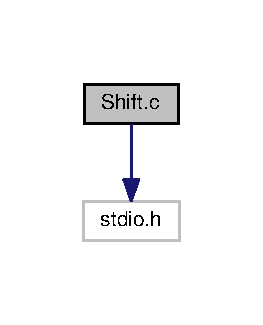
\includegraphics[width=126pt]{Shift_8c__incl}
\end{center}
\end{figure}
\subsection*{Macros}
\begin{DoxyCompactItemize}
\item 
\#define \hyperlink{Shift_8c_ad1f79d9d99776d7353c6659c307c83c6}{M\+A\+XN}~8
\end{DoxyCompactItemize}
\subsection*{Functions}
\begin{DoxyCompactItemize}
\item 
void \hyperlink{Shift_8c_a3a2c5d537ffc22a91b9a68e124f002e6}{printarray} (int a\mbox{[}$\,$\mbox{]}, int n)
\item 
void \hyperlink{Shift_8c_affb07e79872e6229183b3a677c62af08}{shift} (int a\mbox{[}$\,$\mbox{]}, int n, int m)
\item 
int \hyperlink{Shift_8c_a015a3f08ab5b28a934e106bf346e51f6}{getint} (void)
\item 
void \hyperlink{Shift_8c_aca89b2b7d540004183c311d6ce44a5f0}{getarray} (int a\mbox{[}$\,$\mbox{]}, int $\ast$n)
\item 
int \hyperlink{Shift_8c_a840291bc02cba5474a4cb46a9b9566fe}{main} (void)
\end{DoxyCompactItemize}


\subsection{Macro Definition Documentation}
\index{Shift.\+c@{Shift.\+c}!M\+A\+XN@{M\+A\+XN}}
\index{M\+A\+XN@{M\+A\+XN}!Shift.\+c@{Shift.\+c}}
\subsubsection[{\texorpdfstring{M\+A\+XN}{MAXN}}]{\setlength{\rightskip}{0pt plus 5cm}\#define M\+A\+XN~8}\hypertarget{Shift_8c_ad1f79d9d99776d7353c6659c307c83c6}{}\label{Shift_8c_ad1f79d9d99776d7353c6659c307c83c6}


\subsection{Function Documentation}
\index{Shift.\+c@{Shift.\+c}!getarray@{getarray}}
\index{getarray@{getarray}!Shift.\+c@{Shift.\+c}}
\subsubsection[{\texorpdfstring{getarray(int a[], int $\ast$n)}{getarray(int a[], int *n)}}]{\setlength{\rightskip}{0pt plus 5cm}void getarray (
\begin{DoxyParamCaption}
\item[{int}]{a\mbox{[}$\,$\mbox{]}, }
\item[{int $\ast$}]{n}
\end{DoxyParamCaption}
)}\hypertarget{Shift_8c_aca89b2b7d540004183c311d6ce44a5f0}{}\label{Shift_8c_aca89b2b7d540004183c311d6ce44a5f0}

\begin{DoxyCode}
91                                  \{
92     \textcolor{keywordtype}{int} answer;
93     \textcolor{keywordtype}{int} i=0;
94 
95     \textcolor{keywordflow}{do} \{
96       answer = \hyperlink{Shift_8c_a015a3f08ab5b28a934e106bf346e51f6}{getint}();
97       \textcolor{keywordflow}{if} (answer>0 && (i<\hyperlink{Shift_8c_ad1f79d9d99776d7353c6659c307c83c6}{MAXN}))
98     a[i++]=answer;
99     \}\textcolor{keywordflow}{while}(answer>0 && (i<\hyperlink{Shift_8c_ad1f79d9d99776d7353c6659c307c83c6}{MAXN}));
100     *n = i;
101   \}
\end{DoxyCode}


Here is the call graph for this function\+:
\nopagebreak
\begin{figure}[H]
\begin{center}
\leavevmode
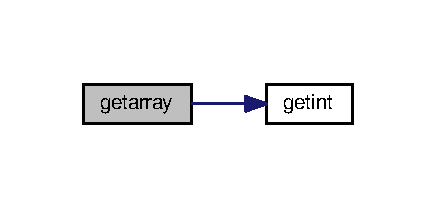
\includegraphics[width=209pt]{Shift_8c_aca89b2b7d540004183c311d6ce44a5f0_cgraph}
\end{center}
\end{figure}


\index{Shift.\+c@{Shift.\+c}!getint@{getint}}
\index{getint@{getint}!Shift.\+c@{Shift.\+c}}
\subsubsection[{\texorpdfstring{getint(void)}{getint(void)}}]{\setlength{\rightskip}{0pt plus 5cm}int getint (
\begin{DoxyParamCaption}
\item[{void}]{}
\end{DoxyParamCaption}
)}\hypertarget{Shift_8c_a015a3f08ab5b28a934e106bf346e51f6}{}\label{Shift_8c_a015a3f08ab5b28a934e106bf346e51f6}

\begin{DoxyCode}
79                   \{
80     \textcolor{keywordtype}{int} answer;
81 
82     printf(\textcolor{stringliteral}{"Please enter a positive integer [<=0 to terminate] : "});
83     scanf(\textcolor{stringliteral}{"%d"}, &answer);
84     \textcolor{keywordflow}{return} answer;
85   \}
\end{DoxyCode}
\index{Shift.\+c@{Shift.\+c}!main@{main}}
\index{main@{main}!Shift.\+c@{Shift.\+c}}
\subsubsection[{\texorpdfstring{main(void)}{main(void)}}]{\setlength{\rightskip}{0pt plus 5cm}int main (
\begin{DoxyParamCaption}
\item[{void}]{}
\end{DoxyParamCaption}
)}\hypertarget{Shift_8c_a840291bc02cba5474a4cb46a9b9566fe}{}\label{Shift_8c_a840291bc02cba5474a4cb46a9b9566fe}

\begin{DoxyCode}
42                \{
43   \textcolor{keywordtype}{int} table[\hyperlink{Shift_8c_ad1f79d9d99776d7353c6659c307c83c6}{MAXN}];  \textcolor{comment}{/* array where we store the sequence */}
44   \textcolor{keywordtype}{int} howmany=0;    \textcolor{comment}{/* number of elements in sequence */}
45   \textcolor{keywordtype}{int} amount;       \textcolor{comment}{/* amount of shift */}
46 
47   \hyperlink{Shift_8c_aca89b2b7d540004183c311d6ce44a5f0}{getarray}(table, &howmany);
48   \textcolor{keywordflow}{if} (howmany==0) \{
49     printf(\textcolor{stringliteral}{"Sorry, you entered the null sequence. Good bye.\(\backslash\)n"});
50   \}\textcolor{keywordflow}{else} \{
51     \textcolor{keywordflow}{do} \{
52       \hyperlink{Shift_8c_a3a2c5d537ffc22a91b9a68e124f002e6}{printarray}(table,howmany);
53       printf(\textcolor{stringliteral}{"By how much do you want to shift[0 to terminate]? "});
54       scanf(\textcolor{stringliteral}{"%d"},&amount);
55       \textcolor{keywordflow}{if} (amount!=0)
56     \hyperlink{Shift_8c_affb07e79872e6229183b3a677c62af08}{shift}(table,howmany,amount);
57     \}\textcolor{keywordflow}{while}(amount!=0);
58   \}
59 \}
\end{DoxyCode}


Here is the call graph for this function\+:
\nopagebreak
\begin{figure}[H]
\begin{center}
\leavevmode
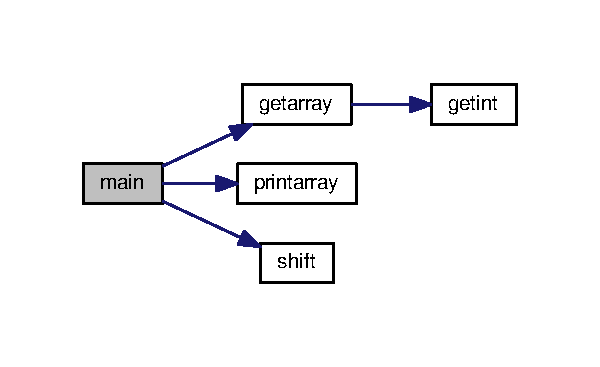
\includegraphics[width=288pt]{Shift_8c_a840291bc02cba5474a4cb46a9b9566fe_cgraph}
\end{center}
\end{figure}


\index{Shift.\+c@{Shift.\+c}!printarray@{printarray}}
\index{printarray@{printarray}!Shift.\+c@{Shift.\+c}}
\subsubsection[{\texorpdfstring{printarray(int a[], int n)}{printarray(int a[], int n)}}]{\setlength{\rightskip}{0pt plus 5cm}void printarray (
\begin{DoxyParamCaption}
\item[{int}]{a\mbox{[}$\,$\mbox{]}, }
\item[{int}]{n}
\end{DoxyParamCaption}
)}\hypertarget{Shift_8c_a3a2c5d537ffc22a91b9a68e124f002e6}{}\label{Shift_8c_a3a2c5d537ffc22a91b9a68e124f002e6}

\begin{DoxyCode}
104                                   \{
105     \textcolor{keywordtype}{int} lcv;
106 
107     \textcolor{keywordflow}{for} (lcv=0;lcv<n;lcv++)\{
108       printf(\textcolor{stringliteral}{"   %d"},a[lcv]);
109     \}
110     printf(\textcolor{stringliteral}{"\(\backslash\)n"});
111   \}\end{DoxyCode}
\index{Shift.\+c@{Shift.\+c}!shift@{shift}}
\index{shift@{shift}!Shift.\+c@{Shift.\+c}}
\subsubsection[{\texorpdfstring{shift(int a[], int n, int m)}{shift(int a[], int n, int m)}}]{\setlength{\rightskip}{0pt plus 5cm}void shift (
\begin{DoxyParamCaption}
\item[{int}]{a\mbox{[}$\,$\mbox{]}, }
\item[{int}]{n, }
\item[{int}]{m}
\end{DoxyParamCaption}
)}\hypertarget{Shift_8c_affb07e79872e6229183b3a677c62af08}{}\label{Shift_8c_affb07e79872e6229183b3a677c62af08}

\begin{DoxyCode}
64                                    \{
65     \textcolor{keywordtype}{int} temp[\hyperlink{Shift_8c_ad1f79d9d99776d7353c6659c307c83c6}{MAXN}];
66     \textcolor{keywordtype}{int} lcv;
67 
68     \textcolor{keywordflow}{if} (m<0)
69       m = n-(abs(m)%n);
70     \textcolor{keywordflow}{for} (lcv=0;lcv<n;lcv++)
71       temp[(lcv+m)%n] = a[lcv];
72     \textcolor{keywordflow}{for} (lcv=0; lcv<n;lcv++)
73       a[lcv]=temp[lcv];
74   \}
\end{DoxyCode}

%--- End generated contents ---

% Index
\backmatter
\newpage
\phantomsection
\clearemptydoublepage
\addcontentsline{toc}{chapter}{Index}
\printindex

\end{document}
